\documentclass{article}
\usepackage[utf8]{inputenc}
\usepackage[spanish]{babel}
\usepackage{listings}
\usepackage{graphicx}
\graphicspath{ {images/} }
\usepackage{cite}

\begin{document}

\begin{titlepage}
    \begin{center}
        \vspace*{1cm}
            
        \Huge
        \textbf{Proyecto De Investigación}
            
        \vspace{0.5cm}
        \LARGE
        Taller Memoria
            
        \vspace{1.5cm}
            
        \textbf{Juan Pablo Palacios Monsalve}
            
      
        
        \vspace{2.0cm}
        \textbf{Prosefor: Augusto Salazar}
      
    
        \textbf{Materia: Informatica II}
      
        \vfill
        
        \vspace{0.8cm}
     
        \Large
        Despartamento de Ingeniería Electrónica y Telecomunicaciones\\
        Universidad de Antioquia\\
        Medellín\\
        Septiembre de 2020
      
    \end{center}
\end{titlepage}

\tableofcontents
\newpage
\section{Introducción}\label{intro}
Dentro de los componentes de nuestros dispositivos inteligentes (computadoras, celulares, tabletas, etc.) se encuentra uno que se encarga de almacenar toda la información que se procesa de manera temporal, la memoria. Podemos pensar en ella como en un refrigerador lleno de toda clase comida (datos).  Pero para que la memoria tenga razón de ser y de uso (Nos vamos a centralizar en su funcionalidad en computadoras), son indispensables componentes como el external data bus (EDB); estos son una fila de cables que interconectan las partes de nuestra computadora, puede ser vistos como las venas en nuestro cuerpo. También está el chip controlador de memoria (MCC) el cual es muy importante, ya que es el puente directo entre la memoria y el procesador. Podemos pensar en el MCC como un nervio de nuestro cerebro conectándose a los recuerdos. El procesador pregunta al MCC por instrucciones y este se dirige a la memoria, toma los datos los envía a través del EDB; pero el MCC no se conecta mágicamente con el procesador para esto también es necesario que entre en escena otro componente importante: el Address bus, que es el encargado de conectar el procesador con el MCC. En resumen para que la memoria funcione de manera armónica con el procesador debe ocurrir lo siguiente:

 ``El Addres bus se encarga de enviar la dirección de los datos, pero no los datos en sí, luego el MCC toma la dirección de los datos, busca los datos en la memoria y entonces los datos se envían a través del EDB hacía el procesador"\cite[Programs and hardware. 5:51]{Coursera}.

\begin{figure}[h]
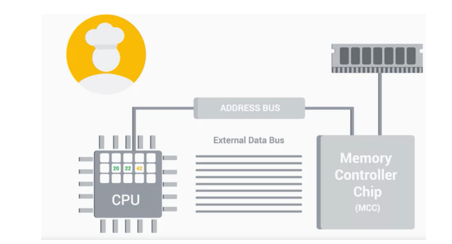
\includegraphics[width=10cm]{Captura.1.PNG}
\centering
\caption{Diagrama de comunicación entre la CPU y la memoria. Tomado de:\cite{Coursera}}
\label{Captura.1.PNG}
\end{figure}
Hay formas más rápidas de obtener datos para nuestro procesador y que este los procese. Por eso hablaré un poco más a fondo y de manera clara de la memoria, de su funcionalidad en sí y de sus tipos. 

\section{Contenido} \label{contenido}

\section{¿Qué es la memoria del computador?}
 ``En muchos sentidos, nuestros recuerdos nos representan, nos ayudan a recordar nuestro pasado, aprender y mantener habilidades, y planificar el futuro. Y para la computadora que actúa como una extensión de nosotros mismos, la memoria juega el mismo papel"\cite[How computer memory works. 00:06]{TEDwebsite} . Es decir, entonces, que la memoria es un dispositivo para almacenar información a corto y largo plazo según sea el caso. 
\vspace{0.2cm}

A corto plazo para tareas inmediatas y a largo plazo para tareas que requieran almacenamiento permanente. Teniendo en cuenta que nosotros como humanos tenemos no uno, sino varios lenguajes para comunicarnos entre nosotros; las computadoras también tienen el suyo, comunicación binaria o sistema de numeración de base 2, esto significa que se comunica unicamente mediante unos y ceros (bits). Entonces la memoria tiene como unidades básicas los bits. Cada uno de estos ocupa un lugar en la denominada celda de memoria (compuestas por transistores, y condensadores) cuyo estado solo puede variar en 1 y 0. Todo lo que vemos en nuestras computadoras ya sea un vídeo, una imagen, texto, no es más que unos y ceros; o sea, los archivos y programas continen millones de bits que se encuentran procesados en la unidad de procesamiento central, que hace las veces de cerebro en nuestra computadora. Al pulsar una tecla,puede ser un procesador de texto por ejemplo, la CPU tomara la decisión de acceder a una de sus facetas mencionadas anteriormente, en este caso a la memoria a corto plazo para recuperar los bits(que también se pueden entender como datos), el tiempo necesario que se toma para esto se conoce como: latencia de memoria. Y como las intrucciones para cada programa deben ser procesadas de manera continua y rapida se tiene la libertad de acceder a cualquier espacio y en cualquier orden dentro de la memoria a corto plazo y es de ahí el nombre a la memoria más conocida de todas. Memoria de acceso aleatorio (RAM), su limitación más importante es que sólo puede almacenar datos siempre y cuando tengan una fuente de alimentación.
\vspace{0.2cm}

Para que los datos no se pierdan una vez se pierda la fuente de alimentación hay que transferirlos en un dispositivo de almacenamiento a largo plazo (memoria a largo plazo). Existen tres tipos principales:
\begin{itemize}
\item Almacenamiento magnetico.
\item Almacenamiento optico.
\item Unidades de estado solido.
\end{itemize}
\section{Tipos de memoria}
\subsection{Memoria de acceso aleatorio (RAM)}
Es la memoria a corto plazo de nuestras computadoras,Almacena datos a los que queremos acceder de forma rapida y continua, esto quiere decir que los datos cambian todo el tiempo, no son permanentes. Al apagar los nuestra computadora los datos almacenados se borran, es decir que la memoria RAM es de caracter volatil.

\begin{figure}[h]
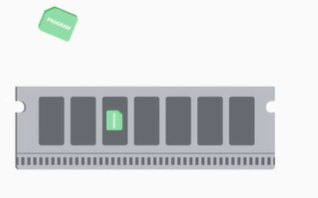
\includegraphics[width=8cm]{Captura.2.PNG}
\centering
\caption{La memoria RAM copia los programas. Tomado de:\cite{Coursera}}
\label{Captura.2.PNG}
\end{figure}
\subsection{Memoria dinámica de acceso aleatorio (DRAM)}
 ``Dicha memoria se llama dinámica porque mantiene una carga por un corto periodo de tiempo antes de perderla y necesita cargarse periodicamente para retener los datos"\cite[How computer memory works. 2:07]{TEDwebsite}. Tiene la capacidad de construir celdas con una gran densidad de posiciones y lograr que funcionen a altas velocidades tanto así que su latencia es muy baja, (del orden de los 100 nanosegundos).

\begin{figure}[h]
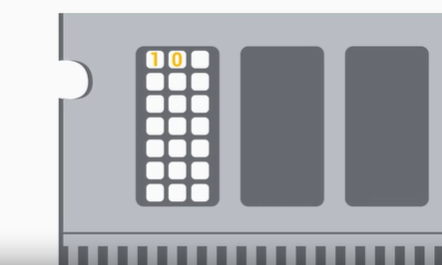
\includegraphics[width=5cm]{dram.PNG}
\centering
\caption{representada con 0 cuando no está cargada, 1 cuando lo está. \centering Tomado de:\cite{Coursera}}
\label{dram.PNG}
\end{figure}
\subsection{DRAM sincrónica}
Este tipo de memoria está sincronizada con la velocidad de reloj de nuestro sistema (esto es la velocidad a la que nuestra CPU realiza un ciclo de operaciones), lo que permite procesar más rápido los datos. Cabe resaltar que SDRAM es la memoria más rapida dentro de un sistema operativo y ocupa más espació que la DRAM.

\begin{figure}[h]
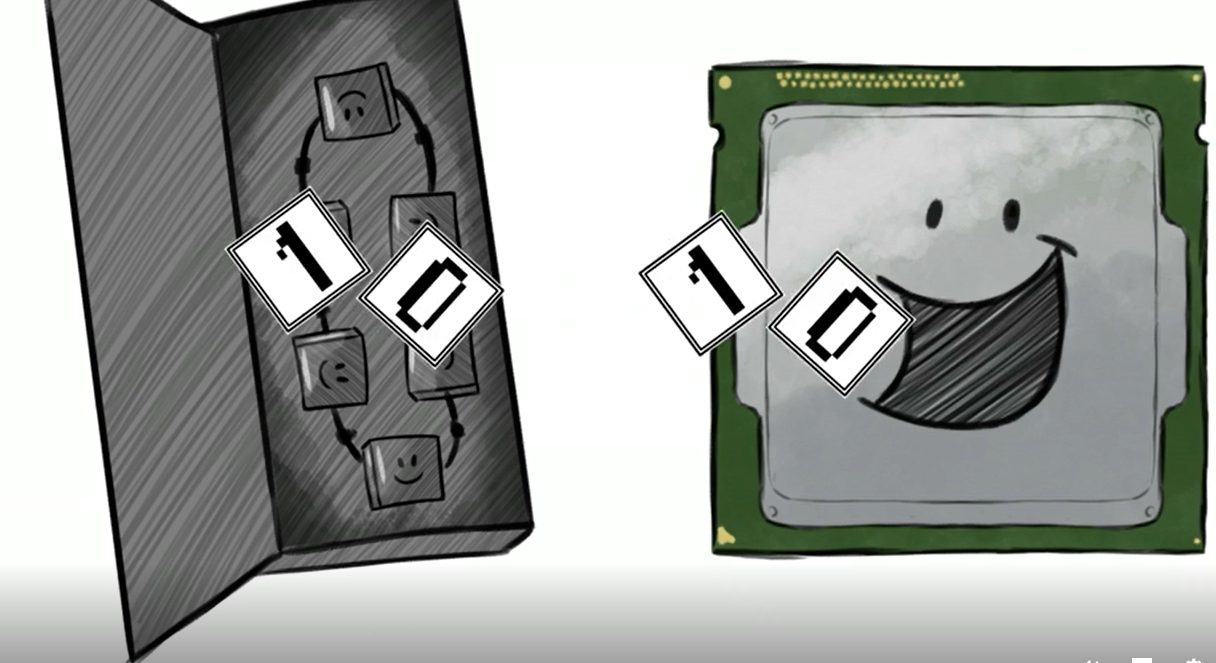
\includegraphics[width=8cm]{SDRAm.PNG}
\centering
\caption{Compuesta por 6 transistores entrelazados que no necesitan recarga. \centering Tomado de:\cite{TEDwebsite}}
\label{SDRAm.PNG}
\end{figure}
\subsection{SDRAM de doble velocidad de datos (DDR)}
Las DDR son versiones mejorada de la SDRAM, son más rápidas, consumen menos energía y cuentan con mayor capacidad. Su versión más actual \textbf{DDR4} es el tipo de memoria a corto plazo más rápido que hay disponible actualmente en el mercado. Una RAM más rápida significa que los programas se pueden ejecutar a mayor rápidez y que pueden ejecutarse más programas al mismo tiempo.
\vspace{0.2cm}
\begin{figure}[h]
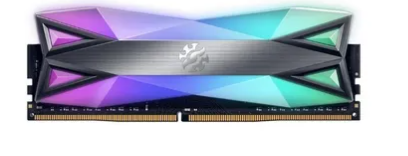
\includegraphics[width=8cm]{DDR4.PNG}
\centering
\caption{DDR4 Gaming RAM. Tomado de:\cite{mercadolibre}. }
\label{DDR4.PNG}
\end{figure}
\newpage
\subsection{Memoria cache}
Está integrada a la CPU y es más pequeña que la RAM; pero nos permite almacenar los datos que usamos más a menudo, algo así como los bolsillos en un pantalon por hacer una analogía, que es donde llevamos las cosas de uso frecuente (celular, llaves, billetera, etc.). Cuenta con tres niveles:
\begin{enumerate}
\item \textbf{L1}: La más rápida de todas.Su función principal es guardar datos importantes de uso frecuente (usuarios,contraseñas).
\item \textbf{L2}: Almacena información recientemente visitada (Sitios Web)
\item \textbf{L3}: Es una memoria especializada en ayudar a mejorar los rendimientos de los niveles L1 y L2.
\end{enumerate}

\begin{figure}[h]
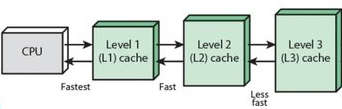
\includegraphics[width=6cm]{Cache.PNG}
\centering
\caption{Jerarquia de la memoria cache. \centering Tomado de:\cite{URUGUAYOC}}
\label{Cache.PNG}
\end{figure}
\subsection{Memoria ROM}
La memoria de sólo lectura (Read Only Memory) es una memoria que como su nombre lo indica sólo es de lectura, esto es, que se puede recuperar; pero no intervenir o modificar.
Tiene tareas de suma importancia como lo son el almacenamiento de software, esto para que la gente no puedan alterarlo por error o interrumpir su funcionamiento. Hoy en día se utiliza para instalar software de arranque como la BIOS (sistema basico de entrada y salida).

\begin{figure}[h]
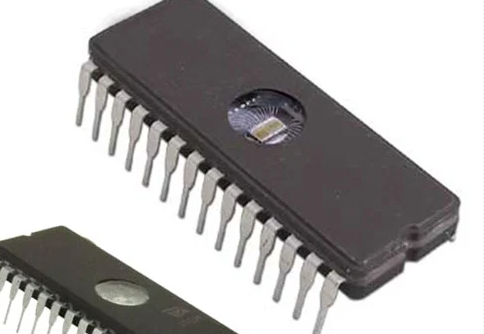
\includegraphics[width=6cm]{ROM.PNG}
\centering
\caption{Memoria ROM.}
\label{ROM.PNG}
\end{figure}

Otra de sus tareas es el almacenamiento de datos; pero estos son datos que no requieren de modificacón alguna cómo los operadores mátematicos y logicos, tablas de consulta, entre otros.
\subsection{Unidad de Disco duro (HDD)}
 También conocido como almacenamiento magnetico. ``Los datos se almacenan según un patron magnetico en un disco giratorio cubierto con una pelicula magnetica"\cite[How computer memory works. 2:57]{TEDwebsite}. Entonces está compuesto basicamente por un disco que gira y brazo mecanico que lee y escribe la información. LA velocidad a la que gira el disco, que permite leer y escribir datos se conoce como RPM (revoluciones por minuto).Por ejemplo un disco duro de 500Gb tendría más o menos una velocidad cercana a 5400 RPM.

La desventaja de estos díscos es que son fragiles por sus partes moviles, puede sufrir daños irreparables y por ende la perdida de información valiosa.

\begin{figure}[h]
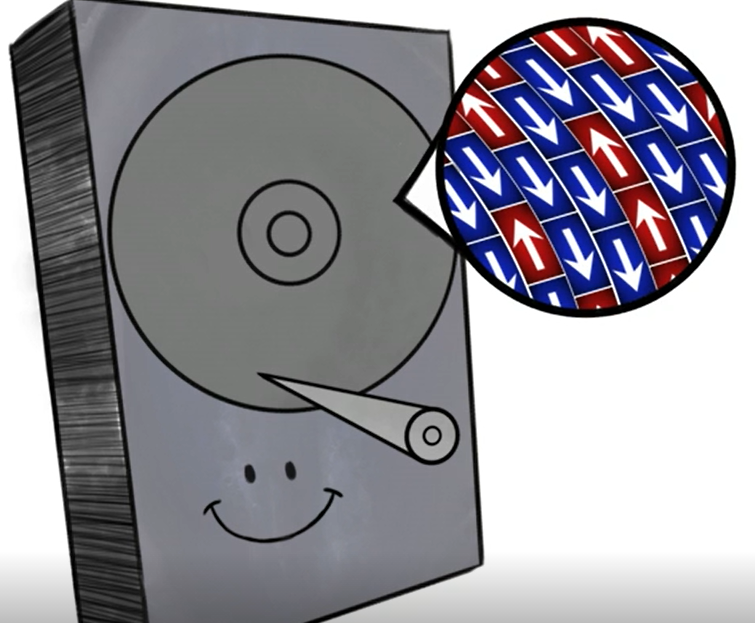
\includegraphics[width=5cm]{HDD.PNG}
\centering
\caption{Hard Drive Disk (HDD). \centering Tomado de: \cite{TEDwebsite}}.
\label{HDD.PNG}
\end{figure}
\subsection{Unidad de Disco duro de estado solido (SDD)}
Podemos pensar en SDD como memorias USB, la información se guarda en microchips. Por tanto los datos viajan a una velocidad mayor superior que en los HDD.`` Esto debido a qué usan transistores de puerta flotante que almacenan datos atrapando o eliminando cargas eléctricas dentro de sus estructuras internas"\cite[How computer memory works. 3:42]{TEDwebsite}.

Al no tener partes moviles se disminuye el riesgo de daño y es mucho más probable que si sufre un daño se pueda salvar la información; pero también son muy caros y además cuentan con menor capacidad de almacenamiento en comparación a los HDD.
\begin{figure}[h]
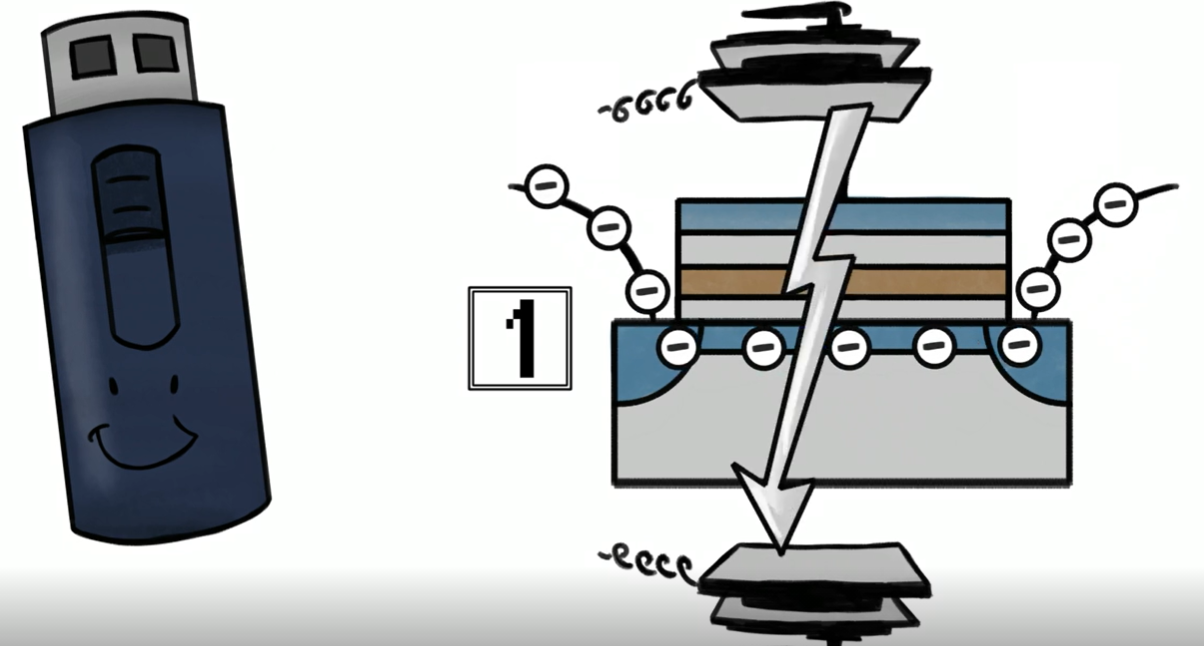
\includegraphics[width=4cm]{SDD.PNG}
\centering
\caption{transistores de puerta flotante de una SDD. Tomado de:\cite{TEDwebsite}}
\label{SDD.PNG}
\end{figure}
\newpage
\section{Gestión de memoria en un computador}
 El SO (sistema operativo) es el encargado de llevar a cabo este proceso. Su principio fundamental es cumplir con su función de gestión por medio de registros para destinar partes de la memoria a los programas que son requeridos en su momento, y a su vez, liberar partes de la misma que no se están usando para que se encuentre disponibles para su almacenamiento. 
\vspace{0.2cm}

\textbf{Caracteristicas}:

\begin{itemize}
\item\textbf{Protección}:  ``es un método para controlar el uso de memoria en una computadora, y es parte esencial de prácticamente todos los sistemas operativos modernos. El principal propósito de la protección de memoria es evitar que un proceso en un sistema operativo acceda a la memoria que no le ha sido asignada"\cite[Unidad 3. Procesos de memoria y almacenamiento]{Sites.Google}.
\item\textbf{Memoria Compartida}:  ``Aunque la memoria utilizada por diferentes procesos suele estar protegida, algunos procesos puede que sí tengan que compartir información y, para ello, han de acceder la misma sección de memoria. La memoria compartida es una de las técnicas más rápidas para posibilitar la comunicación entre procesos"\cite[Unidad 3. Procesos de memoria y almacenamiento]{Sites.Google}.
\item\textbf{Organización Lógica}:  ``Permiten que los programas se escriban como módulos compilables y ejecutables por separado"\cite[Unidad 3. Procesos de memoria y almacenamiento]{Sites.Google}.
\item\textbf{Organización Física}:  ``La memoria suele dividirse en un almacenamiento primario de alta velocidad y uno secundario de menor velocidad.  La gestión de memoria del sistema operativo se ocupa de trasladar la información entre estos dos niveles de memoria"\cite[Unidad 3. Procesos de memoria y almacenamiento]{Sites.Google}.
\end{itemize}
\newpage
\section{¿Qué hace que una memoria sea más rapida que otra?¿Por qué esto es importante?}
 Lo que hace a una memoria más rapida que otras son dos apartados muy imporantes que son: \textbf{la frecuencia} y \textbf{la latencia}.La primera tiene que ver con la velocidad de ciclos en un segundo; mientras más grande sea la frecuencia que tiene una memoria más rapido será la cantidad de ciclos. La segunda se puede entender como el retraso que experimenta la memoria.
\vspace{0.2cm}

Para conocer exactamente la velocidad de latencia hay un número imporante que multiplicado con la frecuencia nos  arroja con exactitud este dato y es el \textbf{cast latency}. El dato de frecuencia viene contramarcado en la parte trasera de nuestros modulos de memoria,sin embargo, ese no es el valor verdadero. Los modulos más actules y comunes que son los DDR, cada modulo tiene dos lineas de datos donde cada linea corre a la mitad de lo que dice el modulo y está si es la frecuencia verdadera. Por ejemplo si tenemos 3000Mhz la frecuecia real será: 1500Mhz. Y como mencione anteriormente usando el Cast de latencia y la frecuencia real podemos encontrar el tiempo de respuesta de nuestros modulos de memoria (velocidad de latencia).Donde los mejores modulos cuentan con una velocidad aproximada  a los 10ns. Esto quiere decir que mientras más nanosegundos haya más lenta es la memoria.
\vspace{0.2cm}

Entonces es importante la rapidez en una memoria porque una mayor frecuencia permite tener transferencia de datos en menos tiempo. En procesos como producción y renderización la velocidad de memoria es un apartado de suma importancia.

\begin{figure}[h]
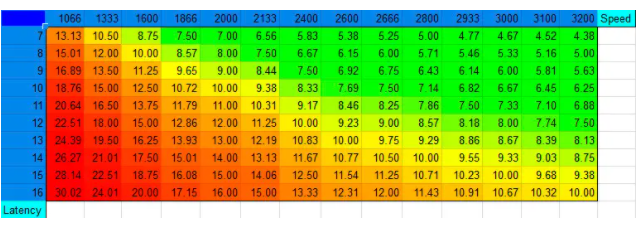
\includegraphics[width=12cm]{latencia.PNG}
\centering
\caption{Frecuencia vs latencia. Tomado de:\cite{Frecuencia}}
\label{latencia.PNG}
\end{figure}
\newpage
\section{Conclusión}
Creemos que la memoria es algo estable y duradero; pero en realidad se degrada con bastante rapidez. La esperanza de vida de estos dispositivos no supera los 10 años de vida util. Con los avances tecnologicos, diseñadores, cientificos e ingenieros se enfrentan con problemas como: tamaño, costo y velocidad. Tratan de explotar al máximo las propiedades físicas de los materiales con la esperanza de crear dispositivos que cumplan con estos requerimientos, eso si siempre sacrificando algún otro apartado del hardware.

 ``Por ahora, la inmortalidad queda fuera del alcance, tanto para los seres humanos como para las computadoras"\cite[How computer memory works. 4:39]{TEDwebsite}.



\newpage
\bibliographystyle{IEEEtran}
\bibliography{references}

\end{document}
